%**************************************%
%*    Generated from PreTeXt source   *%
%*    on 2018-02-07T12:28:10Z    *%
%*                                    *%
%*   http://mathbook.pugetsound.edu   *%
%*                                    *%
%**************************************%
\documentclass[10pt,]{book}
%% Custom Preamble Entries, early (use latex.preamble.early)
%% Inline math delimiters, \(, \), need to be robust
%% 2016-01-31:  latexrelease.sty  supersedes  fixltx2e.sty
%% If  latexrelease.sty  exists, bugfix is in kernel
%% If not, bugfix is in  fixltx2e.sty
%% See:  https://tug.org/TUGboat/tb36-3/tb114ltnews22.pdf
%% and read "Fewer fragile commands" in distribution's  latexchanges.pdf
\IfFileExists{latexrelease.sty}{}{\usepackage{fixltx2e}}
%% Text height identically 9 inches, text width varies on point size
%% See Bringhurst 2.1.1 on measure for recommendations
%% 75 characters per line (count spaces, punctuation) is target
%% which is the upper limit of Bringhurst's recommendations
%% Load geometry package to allow page margin adjustments
\usepackage{geometry}
\geometry{letterpaper,total={340pt,9.0in}}
%% Custom Page Layout Adjustments (use latex.geometry)
%% This LaTeX file may be compiled with pdflatex, xelatex, or lualatex
%% The following provides engine-specific capabilities
%% Generally, xelatex and lualatex will do better languages other than US English
%% You can pick from the conditional if you will only ever use one engine
\usepackage{ifthen}
\usepackage{ifxetex,ifluatex}
\ifthenelse{\boolean{xetex} \or \boolean{luatex}}{%
%% begin: xelatex and lualatex-specific configuration
%% fontspec package will make Latin Modern (lmodern) the default font
\ifxetex\usepackage{xltxtra}\fi
\usepackage{fontspec}
%% realscripts is the only part of xltxtra relevant to lualatex 
\ifluatex\usepackage{realscripts}\fi
%% 
%% Extensive support for other languages
\usepackage{polyglossia}
%% Main document language is US English
\setdefaultlanguage{english}
%% Spanish
\setotherlanguage{spanish}
%% Vietnamese
\setotherlanguage{vietnamese}
%% end: xelatex and lualatex-specific configuration
}{%
%% begin: pdflatex-specific configuration
%% translate common Unicode to their LaTeX equivalents
%% Also, fontenc with T1 makes CM-Super the default font
%% (\input{ix-utf8enc.dfu} from the "inputenx" package is possible addition (broken?)
\usepackage[T1]{fontenc}
\usepackage[utf8]{inputenc}
%% end: pdflatex-specific configuration
}
%% Symbols, align environment, bracket-matrix
\usepackage{amsmath}
\usepackage{amssymb}
%% allow page breaks within display mathematics anywhere
%% level 4 is maximally permissive
%% this is exactly the opposite of AMSmath package philosophy
%% there are per-display, and per-equation options to control this
%% split, aligned, gathered, and alignedat are not affected
\allowdisplaybreaks[4]
%% allow more columns to a matrix
%% can make this even bigger by overriding with  latex.preamble.late  processing option
\setcounter{MaxMatrixCols}{30}
%%
%% Color support, xcolor package
%% Always loaded.  Used for:
%% mdframed boxes, add/delete text, author tools
\PassOptionsToPackage{usenames,dvipsnames,svgnames,table}{xcolor}
\usepackage{xcolor}
%%
%% Semantic Macros
%% To preserve meaning in a LaTeX file
%% Only defined here if required in this document
%% Subdivision Numbering, Chapters, Sections, Subsections, etc
%% Subdivision numbers may be turned off at some level ("depth")
%% A section *always* has depth 1, contrary to us counting from the document root
%% The latex default is 3.  If a larger number is present here, then
%% removing this command may make some cross-references ambiguous
%% The precursor variable $numbering-maxlevel is checked for consistency in the common XSL file
\setcounter{secnumdepth}{3}
%% Environments with amsthm package
%% Theorem-like environments in "plain" style, with or without proof
\usepackage{amsthm}
\theoremstyle{plain}
%% Numbering for Theorems, Conjectures, Examples, Figures, etc
%% Controlled by  numbering.theorems.level  processing parameter
%% Always need a theorem environment to set base numbering scheme
%% even if document has no theorems (but has other environments)
\newtheorem{theorem}{Theorem}[section]
%% Only variants actually used in document appear here
%% Style is like a theorem, and for statements without proofs
%% Numbering: all theorem-like numbered consecutively
%% i.e. Corollary 4.3 follows Theorem 4.2
\newtheorem{lemma}[theorem]{Lemma}
%% Definition-like environments, normal text
%% Numbering is in sync with theorems, etc
\theoremstyle{definition}
\newtheorem{definition}[theorem]{Definition}
%% Example-like environments, normal text
%% Numbering is in sync with theorems, etc
\theoremstyle{definition}
\newtheorem{example}[theorem]{Example}
%% Numbering for inline exercises is in sync with theorems, normal text
\theoremstyle{definition}
\newtheorem{exercise}[theorem]{Exercise}
%% Localize LaTeX supplied names (possibly none)
\renewcommand*{\proofname}{Proof}
\renewcommand*{\chaptername}{Chapter}
%% Figures, Tables, Listings, Named Lists, Floats
%% The [H]ere option of the float package fixes floats in-place,
%% in deference to web usage, where floats are totally irrelevant
%% You can remove some of this setup, to restore standard LaTeX behavior
%% HOWEVER, numbering of figures/tables AND theorems/examples/remarks, etc
%% may de-synchronize with the numbering in the HTML version
%% You can remove the "placement={H}" option to allow flotation and
%% preserve numbering, BUT the numbering may then appear "out-of-order"
%% Floating environments: http://tex.stackexchange.com/questions/95631/
\usepackage{float}
\usepackage{newfloat}
\usepackage[bf]{caption}
%% Adjust figure environment so that it no longer floats
\SetupFloatingEnvironment{figure}{fileext=lof,placement={H},within=section,name=Figure}
%% http://tex.stackexchange.com/questions/16195
\makeatletter
\let\c@figure\c@theorem
\makeatother
%% Raster graphics inclusion, wrapped figures in paragraphs
%% \resizebox sometimes used for images in side-by-side layout
\usepackage{graphicx}
%%
%% More flexible list management, esp. for references and exercises
%% But also for specifying labels (i.e. custom order) on nested lists
\usepackage{enumitem}
%% hyperref driver does not need to be specified, it will be detected
\usepackage{hyperref}
%% configure hyperref's  \url  to match listings' inline verbatim
\renewcommand\UrlFont{\small\ttfamily}
%% Hyperlinking active in PDFs, all links solid and blue
\hypersetup{colorlinks=true,linkcolor=blue,citecolor=blue,filecolor=blue,urlcolor=blue}
\hypersetup{pdftitle={MAS341: Graph Theory}}
%% If you manually remove hyperref, leave in this next command
\providecommand\phantomsection{}
%% If tikz has been loaded, replace ampersand with \amp macro
%% extpfeil package for certain extensible arrows,
%% as also provided by MathJax extension of the same name
%% NB: this package loads mtools, which loads calc, which redefines
%%     \setlength, so it can be removed if it seems to be in the 
%%     way and your math does not use:
%%     
%%     \xtwoheadrightarrow, \xtwoheadleftarrow, \xmapsto, \xlongequal, \xtofrom
%%     
%%     we have had to be extra careful with variable thickness
%%     lines in tables, and so also load this package late
\usepackage{extpfeil}
%% Custom Preamble Entries, late (use latex.preamble.late)
%% Begin: Author-provided packages
%% (From  docinfo/latex-preamble/package  elements)
%% End: Author-provided packages
%% Begin: Author-provided macros
%% (From  docinfo/macros  element)
%% Plus three from MBX for XML characters
\newcommand{\set}[1]{\{1,2,\dotsc,#1\,\}}
 \newcommand{\ints}{\mathbb{Z}}
 \newcommand{\posints}{\mathbb{N}}
 \newcommand{\rats}{\mathbb{Q}}
 \newcommand{\reals}{\mathbb{R}}
 \newcommand{\complexes}{\mathbb{C}}
 \newcommand{\twospace}{\mathbb{R}^2}
 \newcommand{\threepace}{\mathbb{R}^3}
 \newcommand{\dspace}{\mathbb{R}^d}
 \newcommand{\nni}{\mathbb{N}_0}
 \newcommand{\nonnegints}{\mathbb{N}_0}
 \newcommand{\dom}{\operatorname{dom}}
 \newcommand{\ran}{\operatorname{ran}}
 \newcommand{\prob}{\operatorname{prob}}
 \newcommand{\Prob}{\operatorname{Prob}}
 \newcommand{\height}{\operatorname{height}}
 \newcommand{\width}{\operatorname{width}}
 \newcommand{\length}{\operatorname{length}}
 \newcommand{\crit}{\operatorname{crit}}
 \newcommand{\inc}{\operatorname{inc}}
 \newcommand{\HP}{\mathbf{H_P}}
 \newcommand{\HCP}{\mathbf{H^c_P}}
 \newcommand{\GP}{\mathbf{G_P}}
 \newcommand{\GQ}{\mathbf{G_Q}}
 \newcommand{\AG}{\mathbf{A_G}}
 \newcommand{\GCP}{\mathbf{G^c_P}}
 \newcommand{\PXP}{\mathbf{P}=(X,P)}
 \newcommand{\QYQ}{\mathbf{Q}=(Y,Q)}
 \newcommand{\GVE}{\mathbf{G}=(V,E)}
 \newcommand{\HWF}{\mathbf{H}=(W,F)}
 \newcommand{\bfC}{\mathbf{C}}
 \newcommand{\bfG}{\mathbf{G}}
 \newcommand{\bfH}{\mathbf{H}}
 \newcommand{\bfF}{\mathbf{F}}
 \newcommand{\bfI}{\mathbf{I}}
 \newcommand{\bfK}{\mathbf{K}}
 \newcommand{\bfP}{\mathbf{P}}
 \newcommand{\bfQ}{\mathbf{Q}}
 \newcommand{\bfR}{\mathbf{R}}
 \newcommand{\bfS}{\mathbf{S}}
 \newcommand{\bfT}{\mathbf{T}}
 \newcommand{\bfNP}{\mathbf{NP}}
 \newcommand{\bftwo}{\mathbf{2}}
 \newcommand{\cgA}{\mathcal{A}}
 \newcommand{\cgB}{\mathcal{B}}
 \newcommand{\cgC}{\mathcal{C}}
 \newcommand{\cgD}{\mathcal{D}}
 \newcommand{\cgE}{\mathcal{E}}
 \newcommand{\cgF}{\mathcal{F}}
 \newcommand{\cgG}{\mathcal{G}}
 \newcommand{\cgM}{\mathcal{M}}
 \newcommand{\cgN}{\mathcal{N}}
 \newcommand{\cgP}{\mathcal{P}}
 \newcommand{\cgR}{\mathcal{R}}
 \newcommand{\cgS}{\mathcal{S}}
 \newcommand{\bfn}{\mathbf{n}}
 \newcommand{\bfm}{\mathbf{m}}
 \newcommand{\bfk}{\mathbf{k}}
 \newcommand{\bfs}{\mathbf{s}}
 \newcommand{\bijection}{\xrightarrow[\text{onto}]{\text{$1$--$1$}}}
 \newcommand{\injection}{\xrightarrow[]{\text{$1$--$1$}}}
 \newcommand{\surjection}{\xrightarrow[\text{onto}]{}}
 \newcommand{\nin}{\not\in}
 \newcommand{\prufer}{\mbox{prüfer}}
 \DeclareMathOperator{\fix}{fix}
 \DeclareMathOperator{\stab}{stab}
 \DeclareMathOperator{\var}{var}
 \newcommand{\inv}{^{-1}}
\newcommand{\lt}{<}
\newcommand{\gt}{>}
\newcommand{\amp}{&}
%% End: Author-provided macros
%% Title page information for book
\title{MAS341: Graph Theory}
\author{Paul Johnson\\
School of Mathematics and Statistics\\
The University of Sheffield\\
\href{mailto:paul.johnson@sheffield.ac.uk}{\nolinkurl{paul.johnson@sheffield.ac.uk}}
}
\date{2018 Edition}
\begin{document}
\frontmatter
%% begin: half-title
\thispagestyle{empty}
{\centering
\vspace*{0.28\textheight}
{\Huge MAS341: Graph Theory}\\}
\clearpage
%% end:   half-title
%% begin: adcard
\thispagestyle{empty}
\null%
\clearpage
%% end:   adcard
%% begin: title page
%% Inspired by Peter Wilson's "titleDB" in "titlepages" CTAN package
\thispagestyle{empty}
{\centering
\vspace*{0.14\textheight}
%% Target for xref to top-level element is ToC
\addtocontents{toc}{\protect\hypertarget{MAS341}{}}
{\Huge MAS341: Graph Theory}\\[3\baselineskip]
{\Large Paul Johnson}\\[0.5\baselineskip]
{\Large The University of Sheffield}\\[3\baselineskip]
{\Large 2018 Edition}\\}
\clearpage
%% end:   title page
%% begin: copyright-page
\thispagestyle{empty}
\vspace*{\stretch{2}}
\vspace*{\stretch{1}}
\null\clearpage
%% end:   copyright-page
\hypertarget{p-1}{}%
Work builds on notes from previous course, as well as sections of the book Applied Combinatorics by Keller and Trotter, and Discrete Math by Oscar Levin.%
%% begin: preface
\chapter*{Preface}\label{preface-1}
\addcontentsline{toc}{chapter}{Preface}
Course notes for MAS341: Graph Theory at the University of Sheffield.%% end:   preface
%% begin: table of contents
%% Adjust Table of Contents
\setcounter{tocdepth}{1}
\renewcommand*\contentsname{Contents}
\tableofcontents
%% end:   table of contents
\mainmatter
\typeout{************************************************}
\typeout{Chapter 1 Introduction}
\typeout{************************************************}
\chapter[{Introduction}]{Introduction}\label{ch_intro}
\hypertarget{p-2}{}%
The first chapter is an introduction, including the formal definition of a graph and many terms we will use throughout, but more importantly, examples of these concepts and how you should think abotu them.%
\typeout{************************************************}
\typeout{Section 1.1 A first look a graphs}
\typeout{************************************************}
\section[{A first look a graphs}]{A first look a graphs}\label{s_intro_firstlook}
\typeout{************************************************}
\typeout{Subsection 1.1.1 The idea of a graph}
\typeout{************************************************}
\subsection[{The idea of a graph}]{The idea of a graph}\label{subsection-1}
\hypertarget{p-3}{}%
First and foremost, you should think of a graph as a certain type of picture, containing dots and lines connecting those dots, like so:%
\par
\hypertarget{p-4}{}%
We will typically use the letters \(G, H\), or \(\Gamma\) (capital Gamma) to denote a graph.  The ``dots'' or the graph are called \emph{vertices} or \emph{nodes}, and the lines between the dots are called \emph{edges}. Graphs occur frequently in the ``real world'', and typically how to show how something is connected, with the vertices representing the things and the edges showing connections.  \leavevmode%
\begin{itemize}[label=\textbullet]
\item{}\emph{Transit networks:} The London tube map is a graph, with the vertices representing the stations, and an edge between two stations if the tube goes directly between them.  More generally, rail maps in general are graphs, with vertices stations and edges representing line, and road maps as well, with vertices being cities, and edges being roads.%
\item{}\emph{Social networks:} The typical example would be Facebook, with the vertices being people, and edge between two people if they are friends on Facebook.%
\item{}\emph{Molecules in Chemistry:} In organic chemistry, molecules are made up of different atoms, and are often represented as a graph, with the atoms being vertices, and edges representing covalent bonds between the vertices.%
\end{itemize}
%
\par
\hypertarget{p-5}{}%
That is all rather informal, though, and to do mathematics we need very precise, formal definitions.  We now provide that.%
\typeout{************************************************}
\typeout{Subsection 1.1.2 The formal definition of a graph}
\typeout{************************************************}
\subsection[{The formal definition of a graph}]{The formal definition of a graph}\label{subsection-2}
\hypertarget{p-6}{}%
The formal definition of a graph that we will use is the following:%
\begin{definition}[{}]\label{definition-1}
\hypertarget{p-7}{}%
A \emph{graph} \(G\) consists of a set \(V(G)\), called the \emph{vertices} of \(G\), and a set \(E(G)\), called the \emph{edges} of \(G\), of the two element subsets of \(V(G)\)%
\end{definition}
\begin{example}[]\label{example-1}
\hypertarget{p-8}{}%
Consider the water molecule.  It has three vertices, and so \(V(G)=\{O, H1, H2\}\), and two edges \(E(G)=\big\{\{O, H1\},\{O,H2\}\big\}\)%
\end{example}
\hypertarget{p-9}{}%
This formal definition has some perhaps unintended consequences about what a graph is.  Because we have identified edges with the two things they connect, and have a set of edges, we can't have more than one edge between any two vertices.  In many real world examples, this is not the case: for example, on the London Tube, the Circle, District and Picadilly lines all connect Gloucester Road with South Kensington, and so there should be multiple edges between those two vertices on the graph.%
\par
\hypertarget{p-10}{}%
Another consequence is that we require each edge to be a two element subset of \(V(G)\), and so we do not allow for the possibility of an edge between a vertex and itself, often called a \emph{loop}.%
\par
\hypertarget{p-11}{}%
Graphs without multiple edges or loops are sometimes called \emph{simple graphs}.  We will sometimes deal with graphs with multiple edges or loops, and will try to be explicit when we allow this.  Our default assumption is that our graphs are simple.%
\par
\hypertarget{p-12}{}%
Another consequence of the definition is that edges are symmetric, and work equally well in both directions.  This is not always the case: in road systems, there are often one-way streets.  If we were to model Twitter or Instragram as a graph, rather than the symmetric notion of friends we would have to work with ``following''.  To capture these, we have the notion of a \emph{directed graph}, where rather than just lines, we think of the edges as arrows, pointing from one vertex (the source) to another vertex (the target).  To model Twitter or Instagram, we would have an ege from vertex \(a\) to vertex \(b\) if \(a\) followed \(b\).%
\typeout{************************************************}
\typeout{Subsection 1.1.3 Named graphs, and basic examples and concepts}
\typeout{************************************************}
\subsection[{Named graphs, and basic examples and concepts}]{Named graphs, and basic examples and concepts}\label{subsection-3}
\hypertarget{p-13}{}%
Several simple graphs that are frequently referenced have specific names.%
\begin{definition}[{}]\label{definition-2}
\hypertarget{p-14}{}%
The complete graph \(K_n\) is the graph on \(n\) vertices, with an edge between any two distinct vertices.%
\end{definition}
\begin{definition}[{}]\label{definition-3}
\hypertarget{p-15}{}%
The empty graph \(E_n\) is the graph on \(n\) vertices, with no edges.%
\end{definition}
\begin{definition}[{}]\label{definition-4}
\hypertarget{p-16}{}%
The cycle graph \(C_n\) is the graph on \(n\) vertices \(\{v_1,\dots, v_n\}\) with edges \(\{ \{v_1, v_2\}, \{v_2,v_3\},\dots,\{v_{n-1},v_n\}, \{v_n, v_1\}\}\).%
\end{definition}
\begin{definition}[{}]\label{definition-5}
\hypertarget{p-17}{}%
The complelement of a simple graph \(G\), which we will denote \(G^c\), and is sometimes written \(\overline{G}\), is the graph with the same vertex set as \(G\), but \(\{v,w\}\in E(G^c)\) if and only if \(\{v,w\}\notin E(G)\); that is, there is an edge between \(v\) and \(w\) in \(G^c\) if and only if there is not an edge between \(v\) and \(w\) in \(G\)%
\end{definition}
\begin{example}[]\label{example-2}
\hypertarget{p-18}{}%
The empty graph and complete graph are complements of each other; \(K_n^c=E_n\)%
\end{example}
\typeout{************************************************}
\typeout{Section 1.2 Degree and handshaking}
\typeout{************************************************}
\section[{Degree and handshaking}]{Degree and handshaking}\label{s_intro_degrees}
\typeout{************************************************}
\typeout{Subsection 1.2.1 Definition of degree}
\typeout{************************************************}
\subsection[{Definition of degree}]{Definition of degree}\label{subsection-4}
\hypertarget{p-19}{}%
Intuitively, the \emph{degree} of a vertex is the ``number of edges coming out of it''. If we think of a graph \(G\) as a picture, then to find the degree of a vertex \(v\in V(G)\) we draw a very small circle around \(v\), the number of times the \(G\) intersects that circle is the degree of \(v\).  Formally, we have:%
\begin{definition}[{}]\label{definition-6}
\hypertarget{p-20}{}%
Let \(G\) be a simple graph, and let \(v\in V(G)\) be a vertex of \(G\).  Then the \emph{degree of \(v\)}, written \(d(v)\), is the number of edges \(e\in E(G)\) with \(v\in e\). Alternatively, \(d(v)\) is the number of vertices \(v\) is adjacent to.%
\end{definition}
\begin{example}[]\label{example-3}
\end{example}
\hypertarget{p-21}{}%
Note that in the definition we require \(G\) to be a simple graph.  The notion of degree has a few pitfalls to be careful of \(G\) has loops or multiple edges.  We still want to the degree \(d(v)\) to match the intuitive notion of the ``number of edges coming out of \(v\)'' captured in the drawing with a small circle.  The trap to beware is that this notion no longer agrees with ``the number of vertices adjacent to \(v\)'' or the ``the number of edges incident to \(v\)''%
\begin{example}[]\label{example-4}
\end{example}
\typeout{************************************************}
\typeout{Subsection 1.2.2 Extended example: Chemistry}
\typeout{************************************************}
\subsection[{Extended example: Chemistry}]{Extended example: Chemistry}\label{subsection-5}
\hypertarget{p-22}{}%
In organic chemistry, molecules are frequently drawn as graphs, with the vertices being atoms, and an edge betwen two vertices if and only if the corresponding atoms have a covalent bond between them (that is, they share a vertex).%
\begin{example}[Alkanes]\label{example-5}
\end{example}
\hypertarget{p-23}{}%
The location of an element on the periodic table determines the valency of the element -- hence the degree that vertex has in any molecule containing that graph:%
\leavevmode%
\begin{itemize}[label=\textbullet]
\item{}Hydrogen (H) and Fluorine (F) have degree 1%
\item{}Oxygen (O) and Sulfur (S) have degree 2%
\item{}Nitrogen (N) and Phosphorous (P) have degree 3%
\item{}Carbon (C) has degree 4%
\end{itemize}
\hypertarget{p-24}{}%
Usually, most of the atoms involved are carbon and hydrogen. Carbon atoms are not labelled with a C, but just left blank, while hydrogen atoms are left off completely. One can then complete the full structure of the molecule using the valency of each vertex.  On the exam, you may have to know that Carbon has degree 4 and Hydrogen has degree 1; the valency of any other atom would be provided to you%
\par
\hypertarget{p-25}{}%
Graphs coming from organic chemistry do not have to be simple – sometimes there are double bonds, where a pair of carbon atoms have two edges between them.%
\begin{example}[]\label{example-6}
\end{example}
\hypertarget{p-26}{}%
If we know the chemical formula of a molecule, then we know how many vertices of each degree it has.  For a general graph, this information is known as the degree sequence%
\begin{definition}[{Degree sequence}]\label{definition-7}
\hypertarget{p-27}{}%
The degree sequence of a graph is just the list (with multiplicity) of the degrees of all the vertices.%
\end{definition}
\hypertarget{p-28}{}%
So, knowing the chemical composition of a molecule determines the degree sequence of its corresponding graph. However, it is possible that the same set of atoms may be put together into a molecule in more than one different ways. In terms of graphs, this corresponds to “different” graphs that have the same degree sequence.%
\par
\hypertarget{p-29}{}%
An important special case is the constant degree sequence.%
\begin{definition}[{Regular graphs}]\label{definition-8}
\hypertarget{p-30}{}%
A graph \(\Gamma\) is \(d\)-\emph{regular}, or \emph{regular of degree} \(d\) if every vertex \(v\in\Gamma\) has the same degree \(d\), i.e. \(d(v)=d\).%
\end{definition}
\hypertarget{p-31}{}%
As a common special case, a regular graph where every vertex has degree three is called \emph{trivalent}, or \emph{cubic}.%
\par
\hypertarget{p-32}{}%
Some quick examples: \leavevmode%
\begin{enumerate}
\item\hypertarget{li-8}{}The cycle graph \(C_n\) is two-regular%
\item\hypertarget{li-9}{}The complete graph \(K_n\) is \((n-1)\)-regular%
\item\hypertarget{li-10}{}The Petersen graph is trivalent%
\end{enumerate}
%
\begin{exercise}\label{exercise-1}
\end{exercise}
\typeout{************************************************}
\typeout{Subsection 1.2.3 Handshaking lemma and first applications}
\typeout{************************************************}
\subsection[{Handshaking lemma and first applications}]{Handshaking lemma and first applications}\label{subsection-6}
\begin{theorem}[{}]\label{theorem-1}
\hypertarget{p-34}{}%
(Euler's handshaking Lemma)%
%
\begin{equation*}
\sum_{v\in V(G)}d(v)=2|E(G)|
\end{equation*}
\end{theorem}
\begin{proof}\hypertarget{proof-1}{}
\hypertarget{p-35}{}%
We count the ``ends'' of edges two different ways.  On the one hand, every end occurs at a vertex, and at vertex \(v\) there are \(d(v)\) ends, and so the total number of ends is the sum on the left hand side. On the other hand, every edge has exactly two ends, and so the number of ends is twice the number of edges, giving the right hand side.%
\end{proof}
\hypertarget{p-36}{}%
Euler's handshaking lemma will be particularly useful in Section 3, when we study graphs on surfaces, but already it still has some amusing corollaries.%
\typeout{************************************************}
\typeout{Section 1.3 Graph Isomorphisms}
\typeout{************************************************}
\section[{Graph Isomorphisms}]{Graph Isomorphisms}\label{s_intro_isomorphisms}
\hypertarget{p-37}{}%
Generally speaking in mathematics, we say that two objects are "isomorphic" if they are "the same" in terms of whatever structure we happen to be studying.  The symmetric group \(S_3\) and the symmetry group of an equilateral triangle \(D_6\) are isomorphic.  In this section we briefly briefly discuss isomorphisms of graphs.%
\typeout{************************************************}
\typeout{Subsection 1.3.1 Isomorphic graphs}
\typeout{************************************************}
\subsection[{Isomorphic graphs}]{Isomorphic graphs}\label{subsection-7}
\hypertarget{p-38}{}%
It is possible to draw the same graph in the plane in many different ways – e.g., the pentagon \(C_5\), and its complement the five sided star \(C_5^c\) are actually "the same", as indicated by the following labeling of the vertices:%
\begin{definition}[{}]\label{definition-9}
\hypertarget{p-39}{}%
An isomorphism \(\varphi:G\to H\) of simple graphs is a biject \(\varphi:V(G)\to V(H)\) between their vertex sets that preserves the number of edges between vertices.  In other words, \(\varphi(v)\) and \(\varphi(w)\) are adjacent in \(H\)if and only if \(v\) and \(w\) are adjancent in \(G\).%
\end{definition}
\begin{example}[]\label{example-7}
\hypertarget{p-40}{}%
This animated gif shows several graphs isomorphic to the Petersen graph, and demonstrates that they are isomorphic.%
\includegraphics[width=1\linewidth]{images/PetersenIsomorphismAnimated.gif}
\hypertarget{p-41}{}%
Animated gif by \href{https://msollami.com/code/2014/12/24/graph-isomorphisms}{Michael Sollami} for \href{https://www.quantamagazine.org/algorithm-solves-graph-isomorphism-in-record-time-20151214/}{this Quanta Magazine article} on the Graph Isomorphism problem%
\end{example}
\begin{example}[]\label{example-8}
\hypertarget{p-42}{}%
The cycle graph on 5 vertices, \(C_5\) is isomorphic to its complement, \(C_5^c\).  The cycle \(C_5\) is usually drawn as a pentagon, and if we were then going to naively draw \(C_5^c\) we would draw a 5-sided star.%
\end{example}
\hypertarget{p-43}{}%
Although solving the graph isomorphism problem for general graphs is quite difficult, doing it for small graphs by hand is not too bad and is something you must be able to do for the exam.  If the two graphs are actually isomorphic, then you should show this by exhibiting an isomrophism; that is, writing down an explicit bijection between their vertex sets with the desired properties. The most attractive way of doing this, for humans, is to label the vertices of both copies with the same letter set.%
\par
\hypertarget{p-44}{}%
If two graphs are not isomorphic, then you have to be able to prove that they aren't. Of course, one can do this by exhaustively describing the possibilities, but usually it's easier to do this by giving an obstruction – something that is different between the two graphs. One easy example is that isomorphic graphs have to have the same number of edges and vertices. We'll discuss some others in the next section%
\typeout{************************************************}
\typeout{Subsection 1.3.2 Heuristics for showing graphs are or aren't isomorphic}
\typeout{************************************************}
\subsection[{Heuristics for showing graphs are or aren't isomorphic}]{Heuristics for showing graphs are or aren't isomorphic}\label{subsection-8}
\hypertarget{p-45}{}%
Another, only slightly more advanced invariant is the degree sequence of a graph that we saw last lecture in our discussion of chemistry.%
\par
\hypertarget{p-46}{}%
If \(\varphi:G\to H\) is an isomorphism of graphs, than we must have \(d(\varphi(v))=d(v)\) for all vertices \(v\in G\), and since isomorphisms are bijections on the vertex set, we see the degree sequence must be preserved.  However, just because two graphs have the same degree sequences does not mean they are isomorphic.%
\par
\hypertarget{p-47}{}%
Slightly subtler invariants are number and length of cycles and paths.%
\typeout{************************************************}
\typeout{Subsection 1.3.3 Cultural Literacy: The Graph Isomorphism Problem}
\typeout{************************************************}
\subsection[{Cultural Literacy: The Graph Isomorphism Problem}]{Cultural Literacy: The Graph Isomorphism Problem}\label{subsection-9}
\hypertarget{p-48}{}%
This section, as all "Cultural Literacy" sections, is information that you may find interesting, but won't be examined.%
\par
\hypertarget{p-49}{}%
The graph isomorphism problem is the following: given two graphs \(G\) and \(H\), determine whether or not \(G\) and \(H\) are isomorphic. Clearly, for any two graphs \(G\) and \(H\), the problem is solvable: if \(G\) and \(H\) both of \(n\) vertices, then there are \(n!\) different bijections between their vertex sets.  One could simply examine each vertex bijection in turn, checking whether or not it maps edges to edges.%
\par
\hypertarget{p-50}{}%
The problem is interesting because the naive algorithm discussed above is not very efficient: for large \(n\), \(n!\) is absolutely huge, and so in general this algorithm will take a long time.  The question is, is there are a faster way to do check? How fast can we get?%
\par
\hypertarget{p-51}{}%
The isomorphism problem is of fundamental importance to theoretical computer science. Apart from its practical applications, the exact difficulty of the problem is unknown. Clearly, if the graphs are isomorphic, this fact can be easily demonstrated and checked, which means the Graph Isomorphism is in NP.%
\par
\hypertarget{p-52}{}%
Most problems in NP are known either to be easy (solvable in polynomial time, P), or at least as difficult as any other problem in NP (NP complete). This is not true of the Graph Isomorphism problem. In November of last year, Laszlo Babai announced a quasipolynomial-time algorithm for the graph isomorphism problem – you can read about this work in this great popular science article.%
\typeout{************************************************}
\typeout{Section 1.4 Instant Insanity}
\typeout{************************************************}
\section[{Instant Insanity}]{Instant Insanity}\label{s_intro_instantinsanity}
\hypertarget{p-53}{}%
So far, our motivation for studying graph theory has largely been one of philosophy and language.  Before we get too much deeper, however, it may be useful to present a nontrivial and perhaps unexpected application of graph theory; an example where graph theory helps us to do something that would be difficult or impossible to do without it.%
\typeout{************************************************}
\typeout{Subsection 1.4.1 A puzzle}
\typeout{************************************************}
\subsection[{A puzzle}]{A puzzle}\label{subsection-10}
\leavevmode%
\begin{figure}
\centering
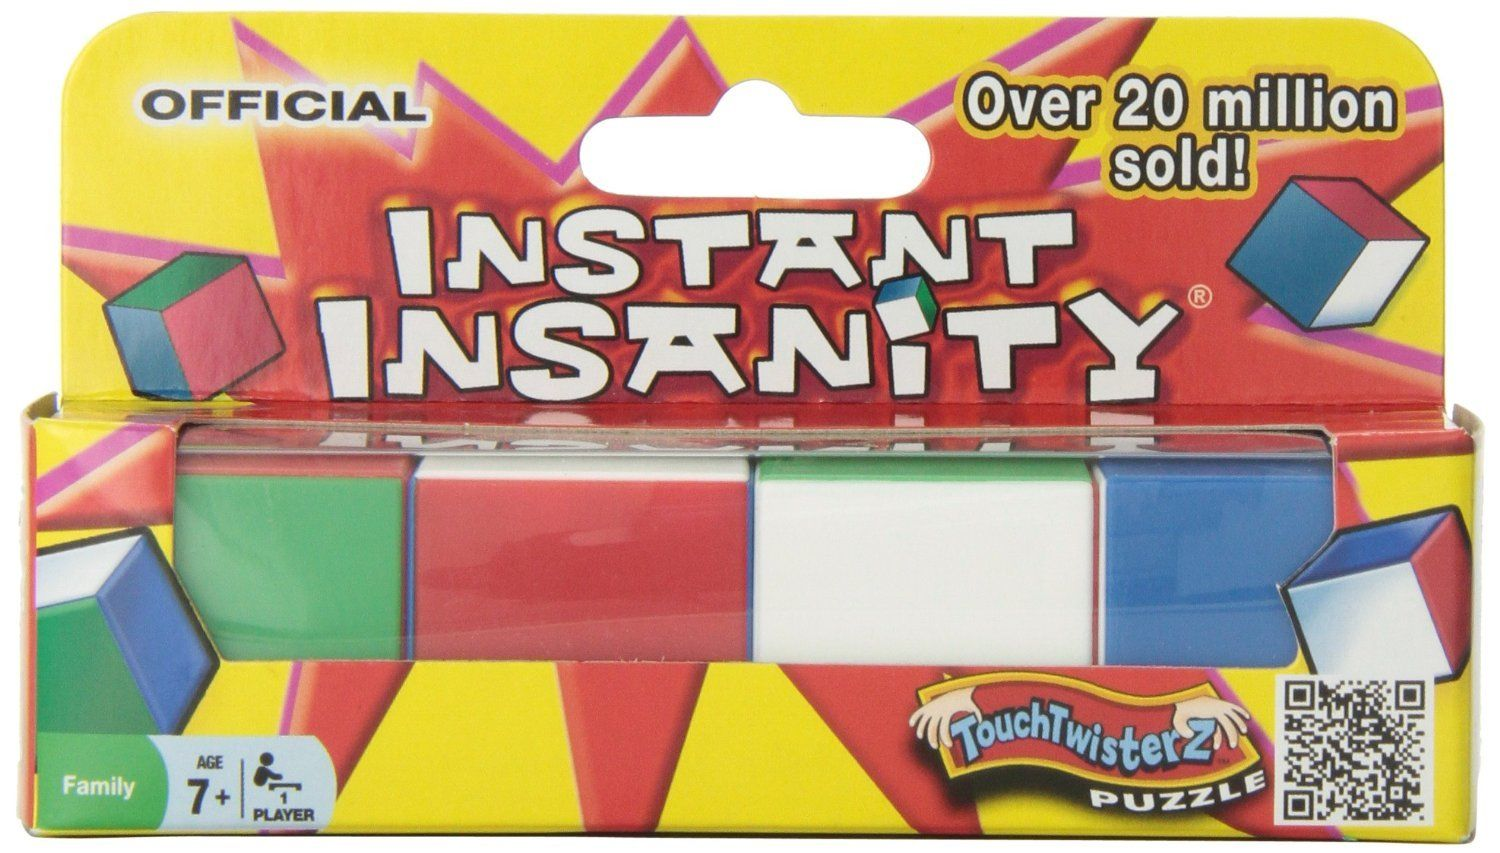
\includegraphics[width=NaN\linewidth]{images/InstantInsanityPackage.JPG}
\caption{Instant Insanity Package\label{figure-1}}
\end{figure}
\hypertarget{p-54}{}%
There is a puazzle marketed under the name "Instant Insanity", one version of which is shown above.  The puzzle is sometimes called "the four cubes problem", as it consists of four different cubes.   Each face of each cube is painted one of four different colours: blue, green, red or yellow. The goal of the puzzle is to line the four cubes up in a row, so that along the four long edges (front, top, back, bottom) each of the four colours appears eactly once.%
\par
\hypertarget{p-55}{}%
Depending on how the cubes are coloured, this may be not be possible, or there may be many such possibilities. In the original instant insanity, there is exactly one solution (up to certain equivalences of cube positions).  The point of the cubes is that there are a large number of possible cube configurations, and so if you just look for a solution without being extremely systematic, it is highly unlikely you will find it.%
\begin{exercise}\label{exercise-2}
\end{exercise}
\hypertarget{p-57}{}%
There are many variations on Instant Insanity, discussions of which can be found \href{http://www.cs.brandeis.edu/\~storer/JimPuzzles/ZPAGES/zzzInstantInsanity.html}{here} and \href{http://www.jaapsch.net/puzzles/insanity.htm}{here}. There’s also a \href{https://www.youtube.com/watch?v=CQ2gHSKZBEw}{commercial} for the game.%
\typeout{************************************************}
\typeout{Subsection 1.4.2 Enter graph theory}
\typeout{************************************************}
\subsection[{Enter graph theory}]{Enter graph theory}\label{subsection-11}
\hypertarget{p-58}{}%
It turns out that the important factor of the cubes is what color is on the opposite side of each face.  Suppose we want face one facing forward.  Then we have four different ways to rotate the cube to keep this the same.  The same face will always appear on the opposite side, but we can get any of the remaining four faces to be on top, say.%
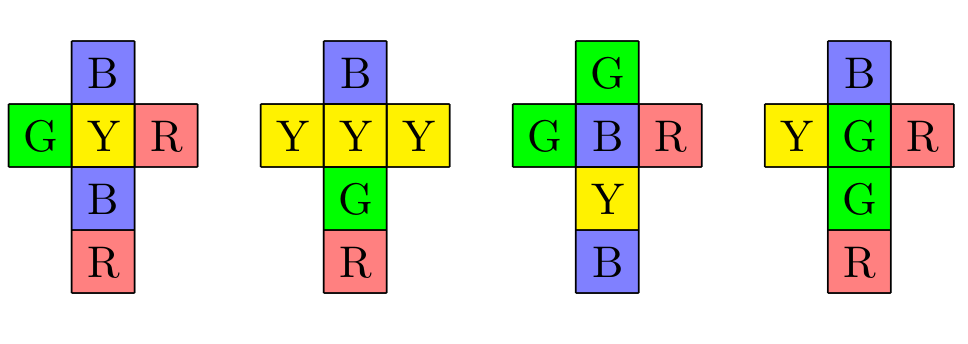
\includegraphics[width=1\linewidth]{images/ImpossibleCubes.png}
\hypertarget{p-59}{}%
Let us encode this information in a graph.   The vertices of the graph will be the four colors, B, G, R and Y. We will put an edge between two colors each time they appear as opposite faces on a cube, and we will label that edge with a number 1-4 denoting which cube the two opposite faces appear. Thus, in the end the graph will have twelve edges, three with each label 1-4. For from the first cube, there will be a loop at B, and edge between G and R, and an edge between Y and R.  The graph corresponding to the four cubes above is the following:%
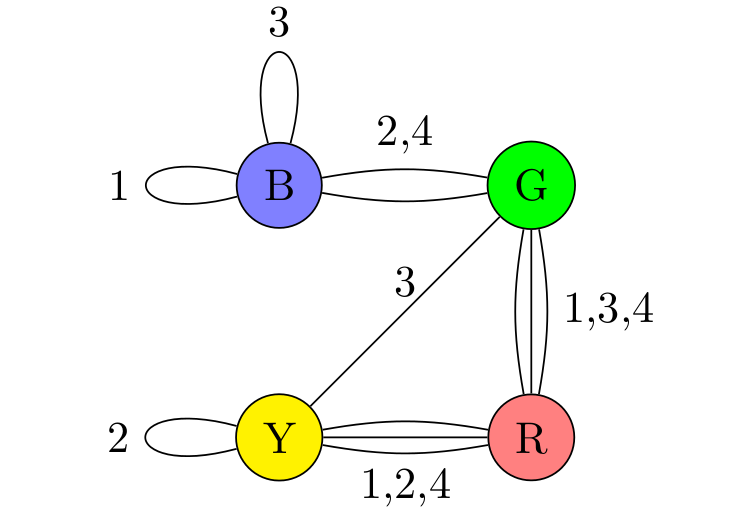
\includegraphics[width=1\linewidth]{images/InstantInsanityImpossibleGraph.png}
\typeout{************************************************}
\typeout{Subsection 1.4.3 Proving that our cubes were impossible}
\typeout{************************************************}
\subsection[{Proving that our cubes were impossible}]{Proving that our cubes were impossible}\label{subsection-12}
\hypertarget{p-60}{}%
We now analyze the graph to prove that this set of cubes is not possible.%
\par
\hypertarget{p-61}{}%
Suppose we had an arrangement of the cubes that was a solution. Then, from each cube, pick the edge representing the colors facing front and back on that cube. These four edges are a subgraph of our original graph, with one edge of each label, since we picked one edge from each cube. Furthermore, since we assumed the arrangement of cubes was a solution of instant insanity, each color appears once on the front face and once on the back. In terms of our subgraph, this translates into asking that each vertex has degree two.%
\par
\hypertarget{p-62}{}%
We can get another subgraph satisfying these two properties by looking at the faces on the top and bottom for each cube and taking the corresponding edges. Furthermore, these two subgraphs do not have any edges in common.%
\par
\hypertarget{p-63}{}%
Thus, given a solution to the instant insanity problem, we found a pair of subgraphs \(S_1, S_2\) satisfying: \leavevmode%
\begin{enumerate}
\item\hypertarget{li-11}{}Each subgraph \(S_i\) has one edge with each label 1,2,3,4%
\item\hypertarget{li-12}{}Every vertex of \(S_i\) has degree 2%
\item\hypertarget{li-13}{}No edge of the original graph is used in both \(S_1\) and \(S_2\)%
\end{enumerate}
 As an exercise, one can check that given a pair of subgraphs satisfying 1-3, one can produce a solution to the instant insanity puzzle.%
\par
\hypertarget{p-64}{}%
Thus, to show the set of cubes we are currently examining does not have a solution, we need to show that the graph does not have two subgraphs satisfying properties 1-3.%
\par
\hypertarget{p-65}{}%
To do, this, we catalog all graphs satisfying properties 1-2. If every vertex has degree 2, either: \leavevmode%
\begin{enumerate}
\item\hypertarget{li-14}{}Every vertex has a loop%
\item\hypertarget{li-15}{}There is one vertex with a loop, and the rest are in a triangle%
\item\hypertarget{li-16}{}There are two vertices with loops and a double edge between the other two vertices%
\item\hypertarget{li-17}{}There are two pairs of double edges%
\item\hypertarget{li-18}{}All the vertices live in one four cycle%
\item\hypertarget{li-19}{}A subgraphs of type 1 is not possible, because G and R do not have loops.%
\end{enumerate}
%
\par
\hypertarget{p-66}{}%
For subgraphs of type 2, the only triangle is G-R-Y, and B does have loops. The edge between Y-G must be labeled 3, which means the loop at B must be labeled 1. This means the edge between G and R must be labeled 4 and the edge between Y and R must be 2, giving the following subgraph:%
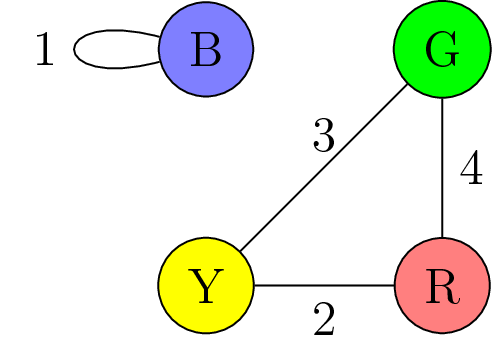
\includegraphics[width=1\linewidth]{images/InstantInsanityImpossibleFirst.png}
\hypertarget{p-67}{}%
For type 3, the only option is to have loops at B and Y and a double edge between G and R. We see the loop at Y must be labeled 2, one of the edges between G and R must be 4, and the loop at B and the other edge between G and R can switch between 1 and 3, giving two possibilities:%
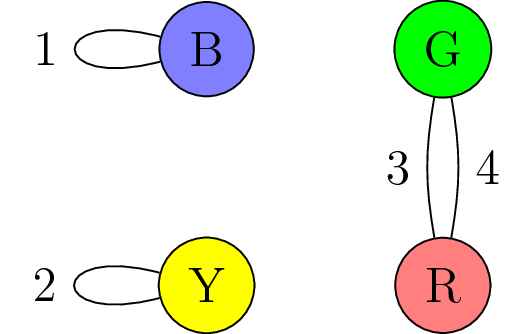
\includegraphics[width=1\linewidth]{images/InstantInsanityImpossibleSecond.png}
\hypertarget{p-68}{}%
and%
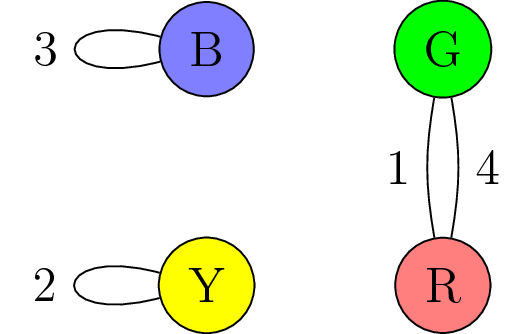
\includegraphics[width=1\linewidth]{images/InstantInsanityImpossibleThird.png}
\hypertarget{p-69}{}%
For subgraphs of type 4, the only option would be to have a double edge between B and G and another between Y and R; however, none of these edges are labeled 3 and this option is not possible.%
\par
\hypertarget{p-70}{}%
Finally, subgraphs of type 5 cannot happen because B is only adjacent to G and to itself; to be in a four cycle it would have two be adjacent to two vertices that aren’t itself.%
\par
\hypertarget{p-71}{}%
This gives three different possibilities for the subgraphs SiSi that satisfy properties 1 and 2. However, all three possibilities contain the the edge labeled 4 between G and R; hence we cannot choice two of them with disjoint edges, and the instant insanity puzzle with these cubes does not have a solution.%
\typeout{************************************************}
\typeout{Chapter 2 Introduction}
\typeout{************************************************}
\chapter[{Introduction}]{Introduction}\label{ch_walks}
\hypertarget{p-72}{}%
In this chapter we investigate walks in graphs.  We first look at some basic definitions and examples, we discuss Dijkstra's algorithm for finding the shortest path between two points in a weighted graph, and we discuss the notions of Eulerian and Hamiltonian graphs.%
\typeout{************************************************}
\typeout{Section 2.1 Walks: the basics}
\typeout{************************************************}
\section[{Walks: the basics}]{Walks: the basics}\label{s_walks_basics}
\hypertarget{p-73}{}%
If the edges in a graph \(\Gamma\) represent connections between different cities, it is obvious to strart planning longer trips that compose several of these connections.  The notion of a \emph{walk} formally captures this definition; the formal notions of \emph{path} and \emph{trail} further ask that we not double back on ourselves or repeat ourselves in certain formally defined ways.%
 \par
\hypertarget{p-74}{}%
Once we've done that, we investigate what it means for a graph to be connected or disconnected.%
\typeout{************************************************}
\typeout{Subsection 2.1.1 Walks and connectedness}
\typeout{************************************************}
\subsection[{Walks and connectedness}]{Walks and connectedness}\label{subsection-13}
\begin{definition}[{Walk}]\label{definition-10}
\hypertarget{p-75}{}%
\(walk\) in a graph \(\Gamma\) is a sequence%
%
\begin{equation*}
v_0, e_1, v_1,e_2, v_2,\dots, v_{n-1}, e_n, v_n
\end{equation*}
\hypertarget{p-76}{}%
where the \(v_i\) are vertices, the \(e_j\) are edges, and the edge \(e_j\) goes between vertices \(v_{j-1}\) and \(v_j\).%
\par
\hypertarget{p-77}{}%
We say that the walk is between vertices \(a=v_0\) and \(b=v_n\)%
\end{definition}
\hypertarget{p-78}{}%
Note that, when the graph \(\Gamma\) does not have multiple edges, it is enough to record just the \(v_i\), but if \(\Gamma\) has multiple edges that just knowing the vertices does not determine the walk.%
\begin{example}[]\label{example-9}
\end{example}
\begin{definition}[{Connected}]\label{definition-11}
\hypertarget{p-79}{}%
We say a graph \(\Gamma\) is \emph{connected} if for any two vertices \(v,w\), there is a walk from \(v\) to \(w\) in \(\Gamma\).%
\end{definition}
\begin{definition}[{Disjoint union}]\label{definition-12}
\hypertarget{p-80}{}%
Given two graphs \(\Gamma_1\) and \(\Gamma_2\), the \emph{disjoint union} \(\Gamma_1\sqcup \Gamma_2\) is obtained by taking the disjoint union of both the vertices and edges of \(\Gamma_1\) and \(\Gamma_2\).  So \(\Gamma_1\sqcup\Gamma_2\) consists of a copy of \(\Gamma_1\) and a copy of \(\Gamma_2\), with no edges in between the two graphs.%
\end{definition}
\begin{definition}[{Disconnected}]\label{definition-13}
\hypertarget{p-81}{}%
A graph \(\Gamma\) is \emph{disconnected} if we can write \(\Gamma=\Gamma_1\sqcup \Gamma_2\) for two proper (i.e., not all of \(\Gamma\)) subgraphs \(\Gamma_1\) and \(\Gamma_2\).%
\end{definition}
\hypertarget{p-82}{}%
We now have a definition for what it means for a graph to be connected, and another for what it means for a graph to be disconnected.  From everday usage of this words, we would certainly hope that a graph is disconnected if and only if it is not connected.  However, it is not immediately clear from the definitions as written that this is the case.%
\begin{lemma}[{}]\label{lemma-1}
\hypertarget{p-83}{}%
The following are equivalent:%
\leavevmode%
\begin{enumerate}
\item\hypertarget{li-20}{}. \(\Gamma\) is connected%
\item\hypertarget{li-21}{}\(\Gamma\) is not disconnected%
\end{enumerate}
\end{lemma}
\begin{proof}\hypertarget{proof-2}{}
\hypertarget{p-84}{}%
1 implies 2: Supppose that \(\Gamma\) is connected, and let \(v, w\in V(\Gamma)\); we want to show that there is a walk from \(v\) to \(w\).%
\par
\hypertarget{p-85}{}%
Define \(S\subset V(\Gamma)\) to be the set of all vertices \(u\in V(\Gamma)\) so that there is a walk from \(v\) to \(u\); we want to show that \(w\in S\).%
\par
\hypertarget{p-86}{}%
First, observe that there are no edges from \(S\) to \(V(\Gamma)\setminus S\).  Suppose that \(e\) was an edge between \(a\in S\) and \(b\in\Gamma\setminus S\).  Since \(a\in S\), by the definition of \(S\) there is a walk \(v=v_0v_1v_2\cdots v_m=a\) from \(v\) to \(a\).  We can add the edge \(e\) to the end of the walk, to get a walk from \(v\) to \(b\), and hence by definition \(b\in S\).%
\par
\hypertarget{p-87}{}%
Now suppose that \(w\notin S\).  Then \(S\) and \(V(\Gamma)\setminus S\) are both nonempty, and by the above there are no edges between them, and so \(\Gamma\) is not connected, a contradiction.%
\par
\hypertarget{p-88}{}%
To prove 2 implies 1, we prove the contrapositive.  If \(\Gamma\) is not connected, then there are two vertices \(v,w\in V(\Gamma)\) so that there is no walk from \(v\) to \(w\).%
\par
\hypertarget{p-89}{}%
Suppose that \(\Gamma=\Gamma_1\sqcup\Gamma_2\), and pick \(v\in V(\Gamma_1), w\in V(\Gamma_2)\).  Any walk from \(v\) to \(w\) starts in \(V(\Gamma_1)\) and ends in \(V(\Gamma_2)\), and so at some point there must be an edge from a vertex in \(\Gamma_1\) to a vertex in \(\Gamma_2\), but there are no such edges \(\square\)%
\end{proof}
\typeout{************************************************}
\typeout{Subsection 2.1.2 Types of Walks}
\typeout{************************************************}
\subsection[{Types of Walks}]{Types of Walks}\label{subsection-14}
\hypertarget{p-90}{}%
Many questions in graph theory ask whether or not a walk of a certain type exists on a graph: we introduce some notation that will be needed for these questions.%
\begin{definition}[{}]\label{definition-14}
\hypertarget{p-91}{}%
We say a walk is \emph{closed} if it starts and ends on the same vertex; i.e., \(v_0=v_n\).  The \emph{length} of a walk is \(n\), the number of edges in it.  The \emph{distance} between two vertices \(v\) and \(w\) is the length of the shortest walk from \(v\) to \(w\), if one exists, and \(\infty\) if one does not exist.%
\end{definition}
\hypertarget{p-92}{}%
It is sometimes convenient to have terminology for walks that don't backtrack on themselves:%
\begin{definition}[{}]\label{definition-15}
\leavevmode%
\begin{enumerate}
\item\hypertarget{li-22}{}If the edges \(e_i\) of the walk are all distinct, we call it a \emph{trail}%
\item\hypertarget{li-23}{}If the vertices \(v_i\) of the walk are all distinct (except possibly \(v_0=v_m\)), we call the walk a \emph{path}.  The exception is to allow for the possibility of closed paths.%
\end{enumerate}
\end{definition}
\begin{lemma}[{}]\label{lemma-2}
\hypertarget{p-93}{}%
Let \(v,w\in V(\Gamma)\).  The following are equivalent:%
\leavevmode%
\begin{enumerate}
\item\hypertarget{li-24}{}There is a walk from \(v\) to \(w\)%
\item\hypertarget{li-25}{}There is a trail from \(v\) to \(w\)%
\item\hypertarget{li-26}{}There is a path from \(v\) to \(w\).%
\end{enumerate}
\end{lemma}
\begin{proof}\hypertarget{proof-3}{}
\hypertarget{p-94}{}%
Obviously, 3 implies 2 which implies 1, as any path is a trail, and any trail is a walk.%
\par
\hypertarget{p-95}{}%
That 1 implies 3 is intuitively obvious: if you repeat a vertex, then you've visited someplace twice, and weren't taking the shortest route.  Let's make this argument mathematically precise.%
\par
\hypertarget{p-96}{}%
Suppose we have a walk \(v=v_0,e_1,\dots, e_m, v_m=w\) that is not a path.  Then, we must repeat some vertex, say \(v_i=v_k\), with \(i\lt k\).  Then we can cut out all the vertices and edges between \(v_i\) and \(v_k\) to obtain a new walk%
%
\begin{equation*}
v=v_0,e_1, v_1,\dots, e_i, v_i, e_{k+1}, v_{k+1}, e_{k+2}, v_{k+2}, \dots, v_m
\end{equation*}
\hypertarget{p-97}{}%
Since \(i \lt k \), the new walk is strictly shorter than our original walk.  Since the length of a walk is finite, if we iterate this process the result must eventually terminate.  That means all our vertices are distinct, and hence is a path.%
\end{proof}
\end{document}